\documentclass[a4paper, 14pt]{extreport}

%\usepackage{showframe} % Отображение границ отступов

\sloppy

% Таблицы
\usepackage{array}
\usepackage{tabularx}
\usepackage{dcolumn}
\usepackage{longtable}
\usepackage{adjustbox}
\usepackage{multirow}

% Кодировка и язык
\usepackage[utf8]{inputenc}
\usepackage[T1,T2A]{fontenc} 
\usepackage[english,russian]{babel}

\usepackage{amsmath}

% Геометрия страницы и графика
\usepackage[left=3cm, right=15mm, top=2cm, bottom=2cm]{geometry} % поля страницы
\usepackage{graphicx}
\usepackage{pdfpages}
\graphicspath{{images/}}

% Прочее
\usepackage[font={normal}]{caption} % настройка подписей к рисункам и таблицам
\usepackage[onehalfspacing]{setspace} % полуторный интервал
\setlength{\parskip}{0cm}
\setlength{\parindent}{1.25cm} 
\usepackage{indentfirst}
\usepackage{hyperref}
\usepackage{float}

% Подписи
\usepackage{ragged2e}
\usepackage{ccaption}
\captiondelim{ — }
\captionstyle{\centering}

% Список источников
\usepackage{csquotes}        
\usepackage[
backend=biber,
hyperref=auto,
sorting=none, % сортировка в порядке встречаемости ссылок
language=auto,
citestyle=gost-numeric,
bibstyle=gost-numeric
]{biblatex}
\addbibresource{biblio.bib}

%Счетчики
\newcounter{mycitecount}  
\usepackage[figure,table,mycitecount]{totalcount}
\usepackage{lastpage}
\AtEveryBibitem{\stepcounter{mycitecount}}

% Замена шрифтов
\usepackage{tempora}

% Настройка подписей к изображениям и таблицам
\captionsetup{format=hang,labelsep=period}

% Настройка заголовков
\usepackage{titlesec}
\titleformat{\chapter}[block]
	{\indent\indent\normalfont\bfseries}{\thechapter}{0.3em}{}
\titleformat{\section}[block]
	{\indent\indent\normalfont\bfseries}{\thesection}{0.3em}{}
\titleformat{\subsection}[block]
	{\indent\indent\normalfont}{\thesubsection}{0.3em}{}
\titlespacing{\chapter}{0pt}{0pt}{0pt}
\titlespacing{\section}{0pt}{20pt}{0pt}
\titlespacing{\subsection}{0pt}{20pt}{0pt}

% Настройка перечислений
\usepackage{enumitem}
\setlist[itemize]{label=\textendash, leftmargin=0mm, itemindent=18mm, itemsep=0mm, parsep=0mm, topsep=0cm}
\setlist[enumerate]{wide=0pt, leftmargin=0mm, itemindent=15mm, itemsep=0mm, parsep=0mm, topsep=0cm,label=\arabic*)}

% Настройка содержания
\usepackage{tocloft}
\renewcommand{\cftbeforechapskip}{0pt}
\renewcommand{\cftbeforetoctitleskip}{-10pt}
\renewcommand{\cftaftertoctitleskip}{8pt}
\renewcommand{\cfttoctitlefont}{\normalfont}
\renewcommand{\cftaftertoctitle}{\hfill}
\renewcommand{\cftchapdotsep}{2}
\renewcommand{\cftchappagefont}{\normalfont}
\renewcommand{\cftsecdotsep}{2}
\renewcommand{\cftsubsecdotsep}{2}
\renewcommand{\cftchapfont}{\normalsize}
\setlength{\cftsecindent}{1em}
\setlength{\cftsubsecindent}{2em}
\setlength{\cftsubsubsecindent}{3em}
\setlength{\cftchapnumwidth}{0.85em}
\setlength{\cftsecnumwidth}{1.7em}
\setlength{\cftsubsecnumwidth}{2.9em}

% Настройка листингов
\usepackage{listings}
\lstdefinestyle{mystyle}{	
	breakatwhitespace=false,         
	breaklines=true,                 
	captionpos=t,                    
	keepspaces=true,                 
	numbers=left,                    
	numbersep=15pt,                  
	showspaces=false,                
	showstringspaces=false,
	showtabs=false,                  
	tabsize=2
}
\lstset{style=mystyle}
\renewcommand{\ttdefault}{cmtt}
\lstset{basicstyle=\small\ttfamily}

\begin{document}	

\includepdf[pages={1-1}]{Titul.pdf}

\chapter*{\hfill РЕФЕРАТ\hfill}

Выпускная квалификационная работа по программе магистратуры \pageref{LastPage} с., \totalfigures{} рис., \totaltables{} табл., \totalmycitecounts{}  источн., 1 прил.
	
\noindent КЛЮЧЕВЫЕ СЛОВА

Объект исследования – 

Предмет исследования – 

Цель работы – 
\newpage
\renewcommand{\contentsname}{\hfill\textbf{СОДЕРЖАНИЕ}\hfill}  
\tableofcontents
	
\chapter*{\hfill ПЕРЕЧЕНЬ СОКРАЩЕНИЙ И ОБОЗНАЧЕНИЙ\hfill}
\addcontentsline{toc}{chapter}{ПЕРЕЧЕНЬ СОКРАЩЕНИЙ И ОБОЗНАЧЕНИЙ}

В настоящей пояснительной записке применяют следующие сокращения и обозначения:

\begin{description}[font=\normalfont,style=multiline,leftmargin=5cm,itemindent=-0.9cm,nosep]
    \raggedright
    
	\item[ВКР]—\ \ \ 
	выпускная квалификационная работа 
    
\end{description}
\chapter*{\hfill ВВЕДЕНИЕ\hfill}
\addcontentsline{toc}{chapter}{ВВЕДЕНИЕ}

Текст введения...
\chapter{Примеры}

\section{Примеры списков и формул}
\subsection{Примеры списков}

Пример ссылок на источники:
\begin{itemize}
	\item книга про Tex \autocite{book};
	\item как писать формулы \autocite{latexformuls}.
\end{itemize}

Пример нумерованного списка:
\begin{enumerate}
	\item первый пункт;
	\item второй пункт.
\end{enumerate}

\subsection{Примеры формул}

Формула в тексте $\forall x \in X, \quad \exists y \leq \epsilon$.

Формула отдельно \ref{formula:example1}:
\begin{equation}	
	\rho(x,x')=\sqrt[r]{\sum_{i}^{n}(x_i-x_i')^P}
	\label{formula:example1}
\end{equation}

\section{Примеры рисунков и таблиц}

Пример рисунка изображен на рисунке \ref{fig:example1}.
\begin{figure}[h!]
	\centering
	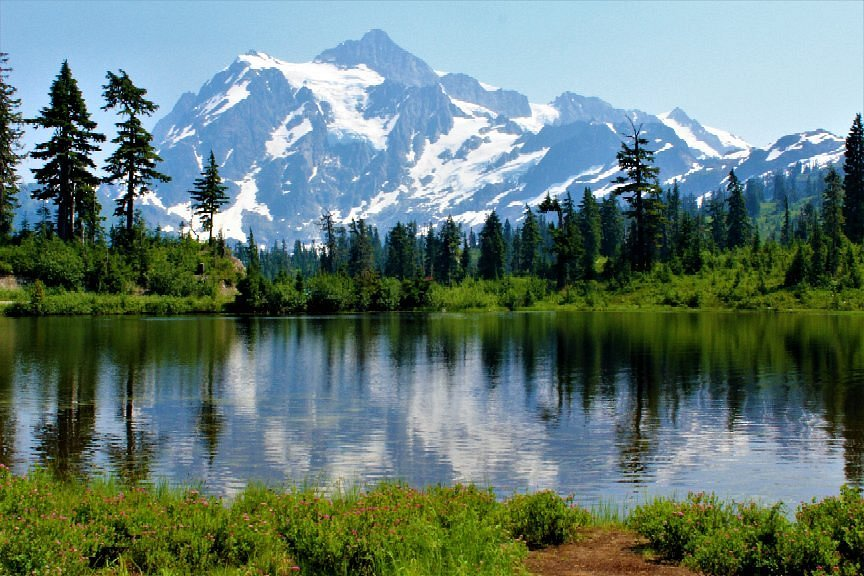
\includegraphics[width=0.7\textwidth]{example1.jpg}
	\caption{Пример рисунка}
	\label{fig:example1}
\end{figure}

Пример таблицы в таблице \ref{table:example1}.

\begin{table}[h!]
\captionstyle{\justifying}
	\caption{Пример таблицы}
		\begin{adjustbox}{width=1\textwidth}
			\small
			\begin{tabular}{|m{3.9cm}|l|m{3cm}|}
				\hline
				\textbf{Колонка 1} & \textbf{Колонка 2} & \textbf{Колонка 3} \\ \hline
				поле 1.1 & поле 2.1 & поле 3.1 \\ \hline
				поле 1.2 & поле 2.2 & поле 3.2 \\ \hline
				поле 1.3 & поле 2.3 & поле 3.3 \\ \hline
			\end{tabular}
		\end{adjustbox}	
	\label{table:example1}
\end{table}
\chapter*{\hfill ЗАКЛЮЧЕНИЕ\hfill}
\addcontentsline{toc}{chapter}{ЗАКЛЮЧЕНИЕ}

Текст заключения...

\newpage
\addcontentsline{toc}{chapter}{СПИСОК ИСПОЛЬЗОВАННЫХ ИСТОЧНИКОВ}
\printbibliography[%{}
	title={\hfill СПИСОК ИСПОЛЬЗОВАННЫХ ИСТОЧНИКОВ\hfill}
]

\chapter*{\hfill ПРИЛОЖЕНИЕ А\hfill}
\refstepcounter{chapter}
\addcontentsline{toc}{chapter}{ПРИЛОЖЕНИЕ А}

\lstinputlisting[language=Python, caption={Файл script.py}]{listing_files/script.py}

\end{document}